\section{Аппаратное обеспечение}
\label{sec:hardware}


\subsection{\SDR-приемник}

\sdr\ (\SDR) --- это разновидность радиосистем, в которых компоненты, традиционно реализуемые аппаратно, замещены программными модулями.
В идеале, из аналоговых устройств хотелось бы оставить только антенну и подключенный к ней аналого-цифровой преобразователь. Все остальные манипуляции с сигналом осуществлялись бы программно. Эта схема обеспечила бы максимальную гибкость и универсальность. Большую часть приемо-передающего тракта можно было бы модифицировать простым обновлением прошивки устройства.
Однако, в настоящее время удовлетворительная частота и точность работы ЦАП и АЦП может быть достигнута только с помощью физических эффектов, таких как интерференция и резонанс. Чтобы привести сигнал к промежуточной частоте используется супергетеродинный приемник. Эти требования увеличивают аналоговую прослойку между антенной и программным обеспечением, но она универсальна и не накладывает концептуальных ограничений на типы принимаемых сигналов.

\begin{figure}[h]
  \centering
  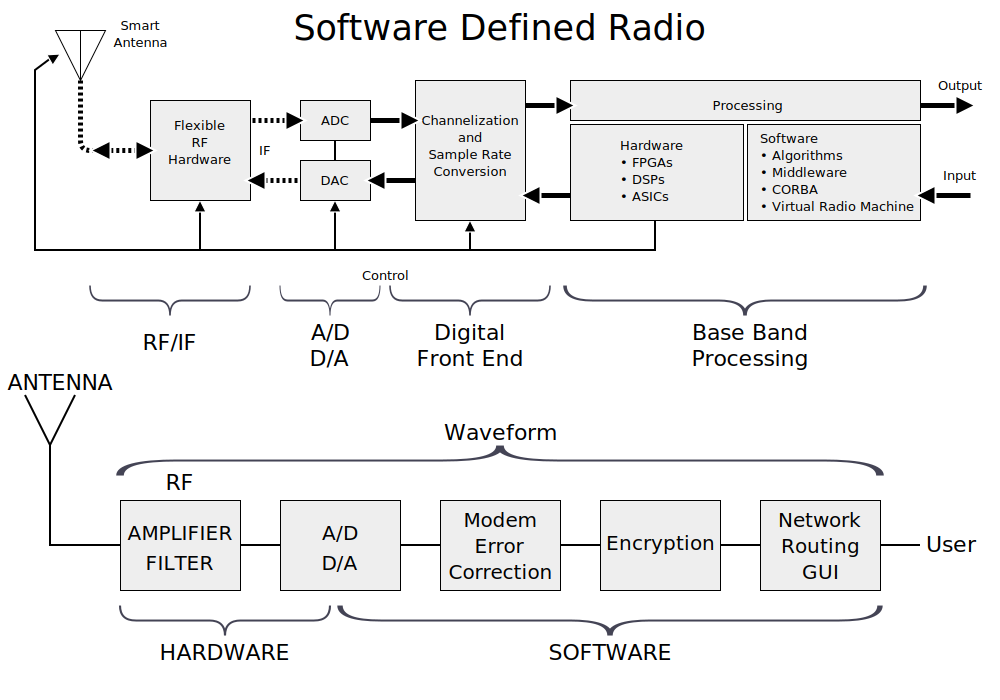
\includegraphics[width=0.8\textwidth]{hardware/sdr_pipeline}
  \caption{Схема работы приемно-передающего тракта \SDR\ \cite{sdr_wiki}}
  \label{fig:hardware:sdr_pipeline}
\end{figure}

Идея \SDR\ не нова --- разработки ведутся с конца \Romannum{20} века. Тогда они не были доступны широкой публике, а программные компоненты создавались для конкретной компьютерной архитектуры. Данные факторы ограничивали развитие этой области радиотехники в основном военными целями.

Положение дел изменилось в 2010 году, когда радиолюбители обнаружили, что ТВ-тюнер Realtek 2832U осуществляет обработку принимаемого сигнала программно. Спецификация платы и протокол взаимодействия ее компонент не были доступны публично, поэтому в следующие годы любители занимались его реверс-инжинирингом. Итогом их действий стала плата на основе вышеупомянутого ТВ-тюнера, способная принимать сигнал с антенны и передавать его комплексное представление приложениям через USB порт.

Стоимость такого устройства невелика --- от \$10 до \$20. Для сравнения, традиционные радиосредства, обладающие сравнимыми характеристиками стоили от \$300 и выше, при том что они поддерживали только несколько протоколов связи. Этот факт дал начало масштабному проникновению \SDR\ в круг энтузиастов. В последние годы это направление бурно развивается, появляются как прикладные приложения, так и аппаратные средства с усовершенствованными характеристиками. В дипломном проекте использовался модифицированный DVB-T тюнер R820T2 (\autoref{fig:hardware:rtl_sdr}).

\begin{figure}[h]
  \centering
  \begin{subfigure}{0.45\textwidth}
    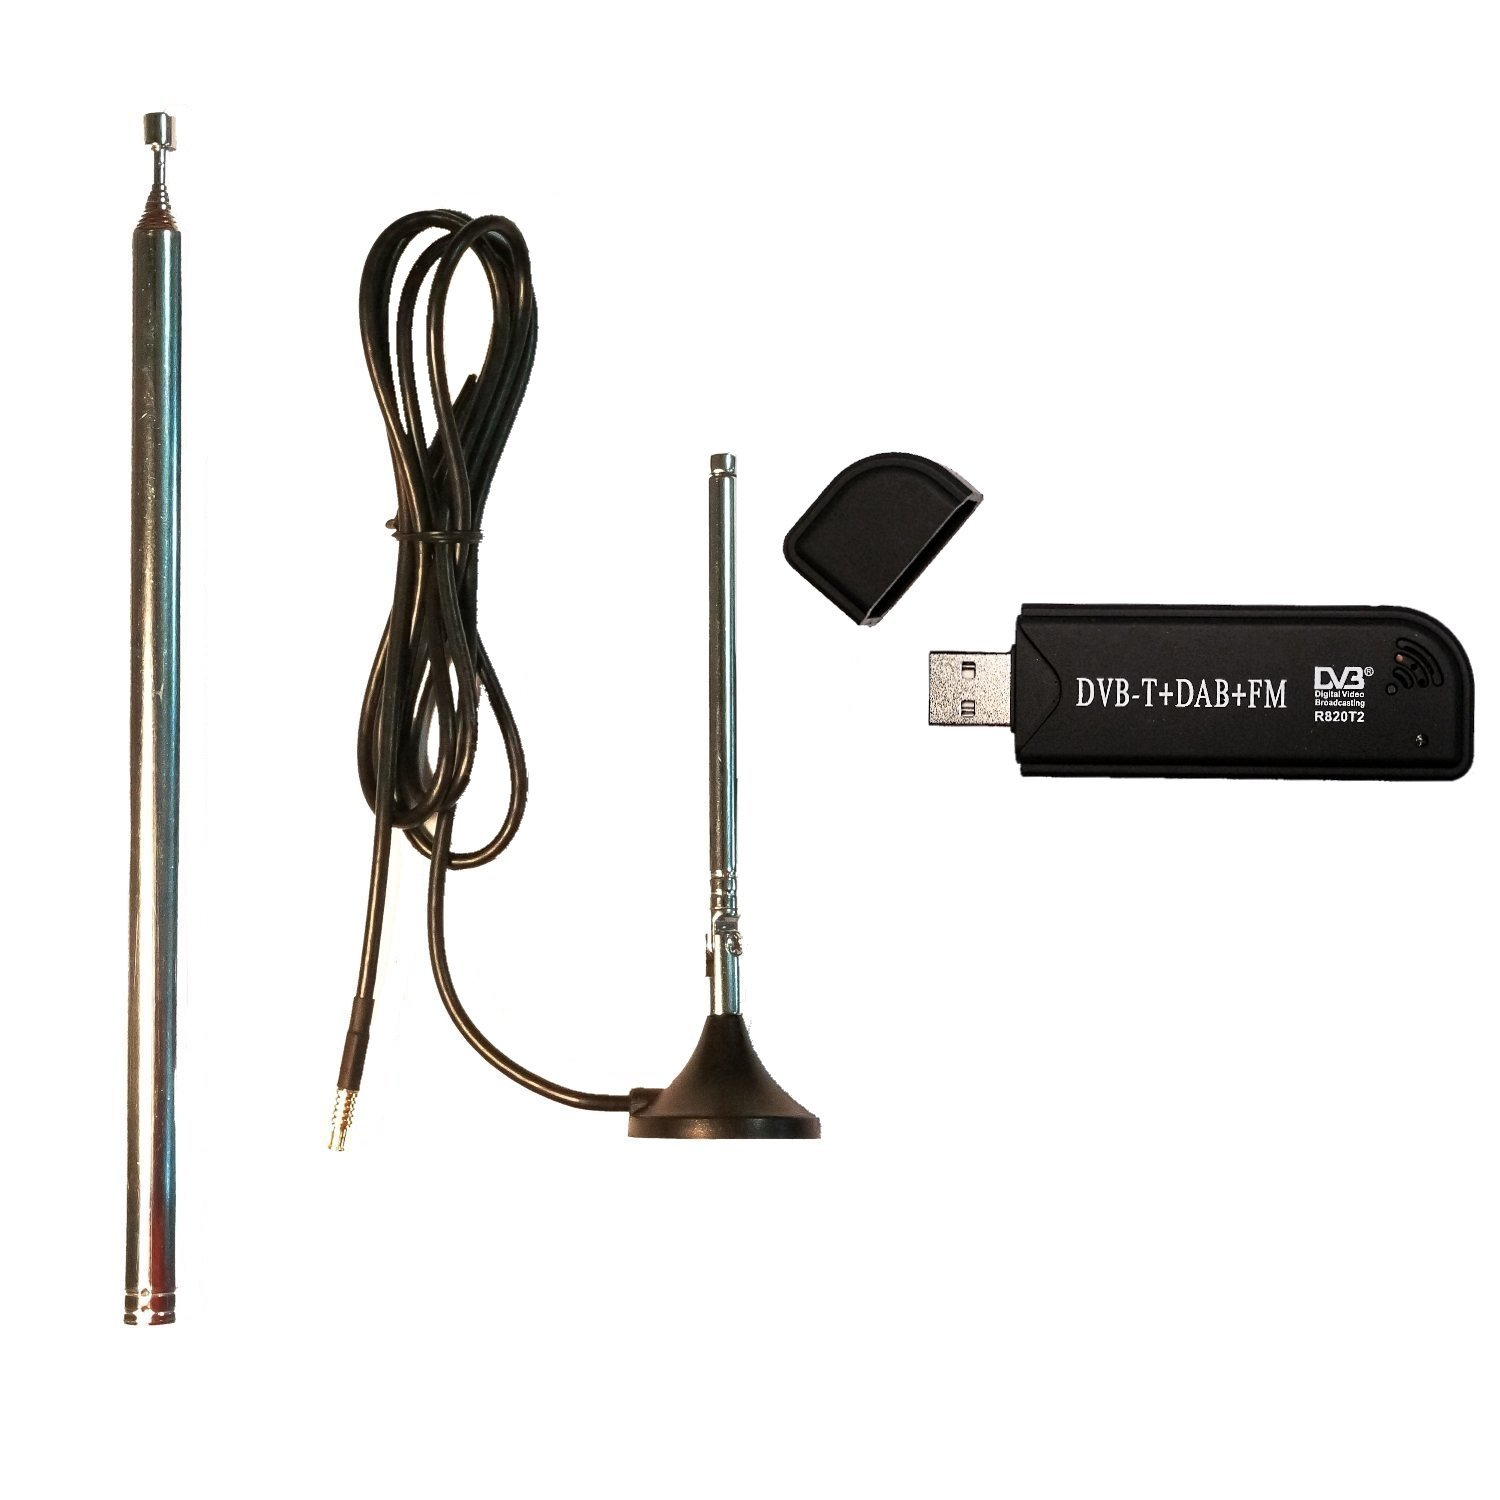
\includegraphics[width=\textwidth]{hardware/rtl_sdr_set}
    \caption{}
    \label{fig:hardware:rtl_sdr_set}
  \end{subfigure}
  \begin{subfigure}{0.45\textwidth}
    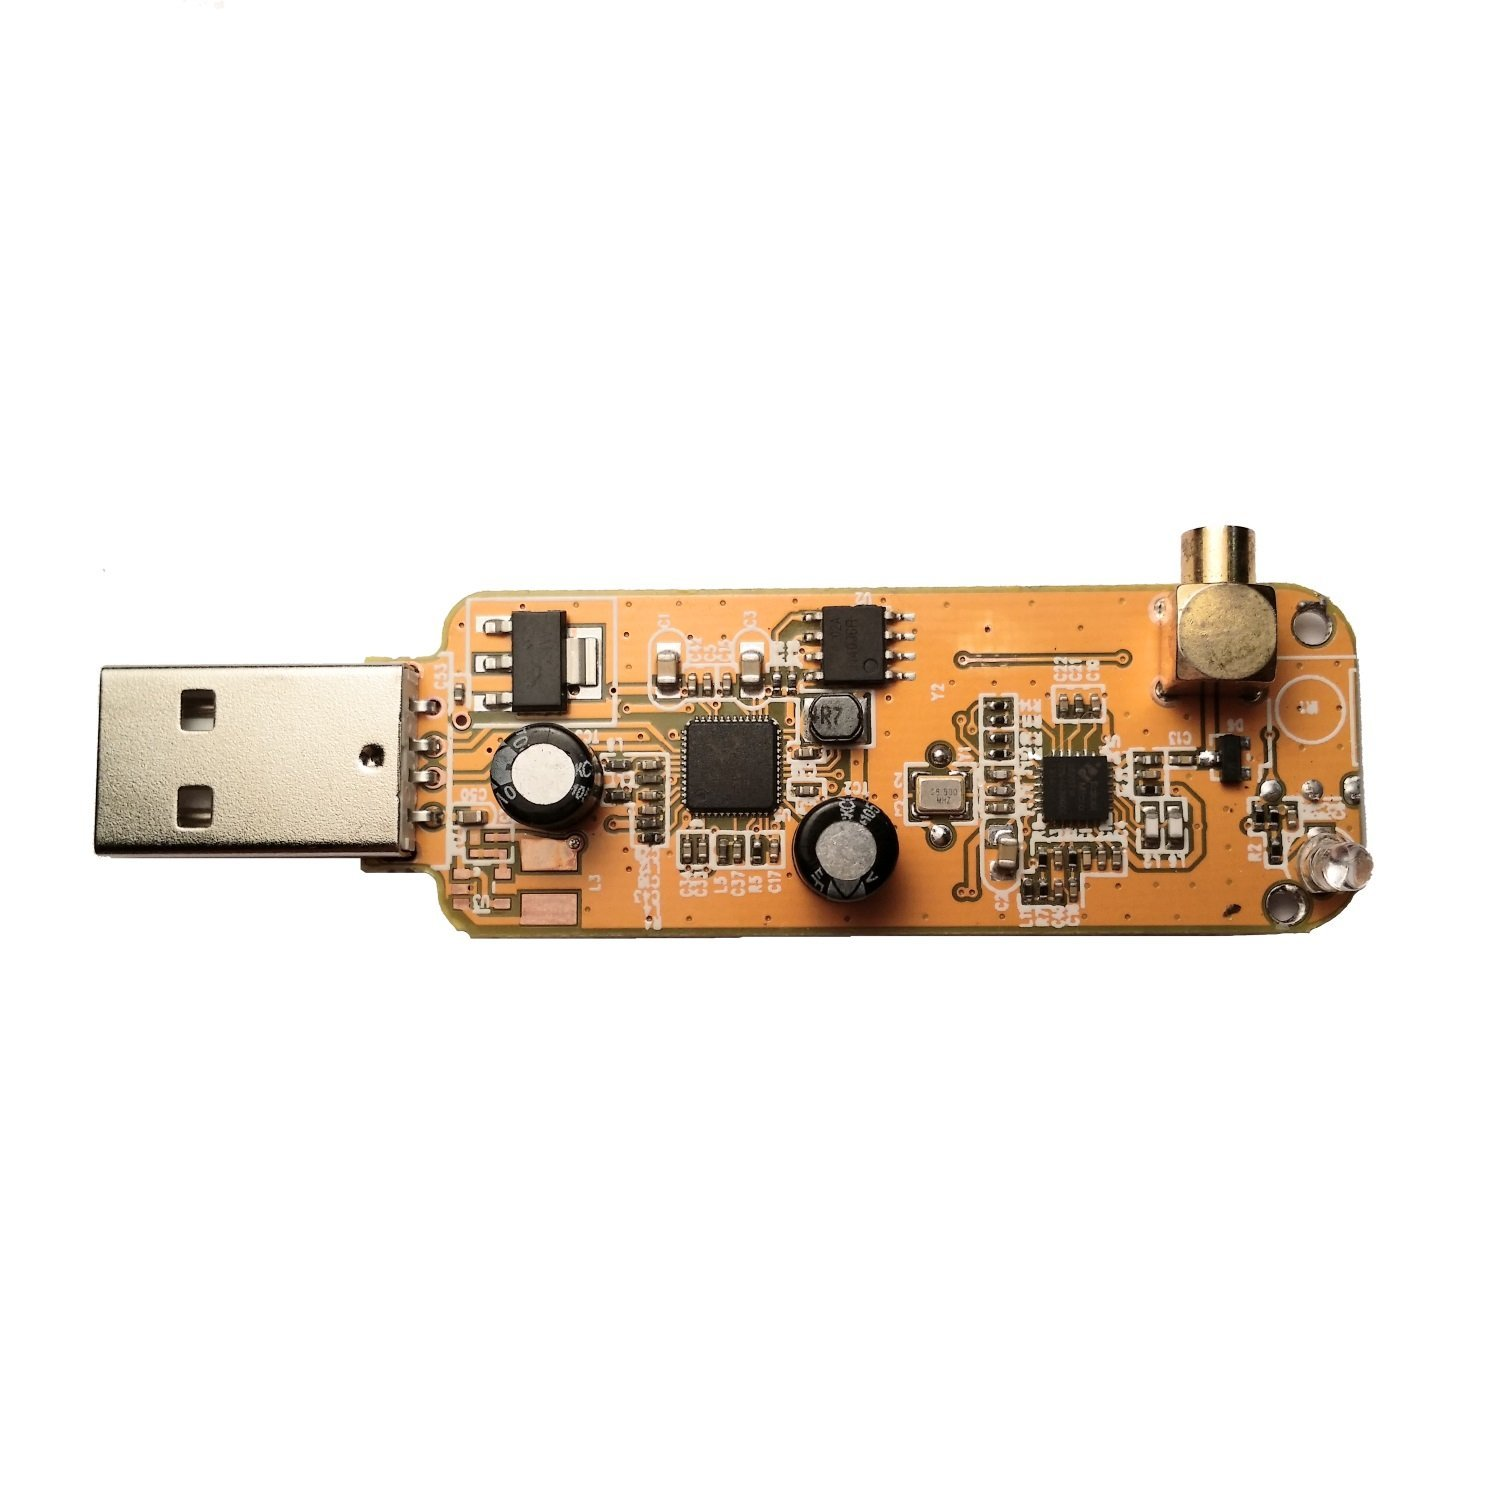
\includegraphics[width=\textwidth]{hardware/rtl_sdr_stripped}
    \caption{}
    \label{fig:hardware:rtl_sdr_stripped}
  \end{subfigure}
  \caption{Готовый к использованию комплект \sdr\ (\subref{fig:hardware:rtl_sdr_set}), внешний вид тюнера без пластикового корпуса (\subref{fig:hardware:rtl_sdr_stripped})}
  \label{fig:hardware:rtl_sdr}
\end{figure}

Определяющим фактором эффективности \SDR\ являются параметры ЦАП и АЦП. Они задают максимальную ширину рабочей полосы частот. В используемом устройстве она ограничена примерно двумя мегагерцами. Это не позволяет использовать его, например, для полноценного приема спутникового телевидения, полоса частот которого шире \SI{2}{\mega\hertz}. В них помещается только звук и черно-белое изображение. Теоретически, можно использовать несколько синхронизированных приемников для увеличения общей ширины полосы, но на практике из-за сложности синхронизации обычно производят замену преобразователей на более мощные.

\subsection{Антенна}

Выбор антенны очень важен для достижения наилучшего качества и дальности передачи. Но мне нужен только прием, поэтому задача значительно упрощается.
В комплект поставки \SDR\ входили две телескопических штыревых антенны длиной до \SI{31.5}{см} и \SI{1.5}{м}. Для исследовательских целей их оказалось достаточно.

Длина антенны прямо пропорциональна максимальной длине волны, которую можно на нее принять. Полтора метра хватает на заявленный диапазон работы Realtek R820T2 --- от \SI{24}{\mega\hertz} до \SI{1.7}{\giga\hertz}.

Достаточно большая полоса частот ниже меньшей границы не может быть использована со стандартными средствами. Но их можно заменять и радиолюбители предлагают использовать в качестве антенны для длинных волн кусок кабеля, вывешенный за окно. Качество приема будет не идеальным, но он закроет неприятную "дыру" ниже \SI{24}{\mega\hertz} в рабочем спектре.

Верхняя граница обусловлена характеристиками преобразователя к промежуточной частоте --- целевое использование устройства было ТВ-тюнером, поэтому оно просто не было спроектировано для работы вне своего диапазона. Сейчас на рынке имеется большое число "чистокровных" \SDR\ со значительно лучшими техническими характеристиками.


\subsection{Субдискретизация}

Как было упомянуто, верхняя граница рабочего диапазона частот находится немногим ниже двух гигагерц, при том что частота дискретизации устройства всего-лишь \SI{2.6}{\mega\sample\per\second} (\num{2.6} миллиона семплов в секунду). Из теоремы Котельникова (Найквиста-Шеннона) следует, что восстановить аналоговый сигнал по дискретной выборке его моментальных значений (семплов) можно только тогда, когда частота дискретизации превышает максимальную частоту компонент сигнала не менее чем в два раза. Следовательно, при частоте дискретизации равной \SI{2.6}{\mega\sample\per\second} получилось бы оцифровать сигнал частотой не более \SI{1.3}{\mega\hertz}. Это так для реальных семплов и сигнала, лежащего в основной полосе частот, но в нашем случае инженерные приемы позволяют работать с этим ограничением.

Во первых, обычно нас интересует не весь диапазон частот от нуля до максимальной, а только определенная полоса, например, \SI{50}{\kilo\hertz} в случае узкополосной FM связи. Если бы она начиналась с нулевой частоты, то никаких технических проблем бы не возникло, но FM диапазон находится как правило выше семидесяти мегагерц и напрямую достать до этой полосы не получается.

В этом случае используется переход к промежуточной частоте. Этот метод основывается на том, что при смешивании двух сигналов с частотами $f_0$ и $f_1$ возникают сигналы с частотами $f_0 - f_1$ и $f_0 + f_1$. Таким образом, можно смешать целевой и близкий к нему сигналы, чтобы "сместить" интересующую нас полосу к нулевой частоте, а затем применить полосовой фильтр, для удаления лишней информации. Конечно, точные значения исходного сигнала теряются, но его по-прежнему можно демодулировать и извлечь полезные данные --- промежуточная частота сохраняет амплитуду и относительную мгновенную частоту.

Во вторых, \SDR\ представляет сигнал в комплексной форме, из-за чего минимальная частота, требуемая теоремой Котельникова, уменьшается вдвое. Комплексный сигнал более "насыщен" информацией. Отрицательные частоты в нем не дублируют положительные. Правда, для получения одного значения нужно иметь два реальных. Поэтому при сравнении АЦП, работающих с комплексным и реальным представлением, можно сказать, что у первых эффективная частота дискретизации в два раза выше номинальной.

Но даже применение этих методов не спасает от ограничения рабочего диапазона частот, который определяется характеристиками гетеродина. Чтобы поднять этот потолок нужно генерировать стабильные колебания на очень высоких частотах. Бюджетные устройства пока не могут позволить себе элементов такого качества.


\subsection{Сравнительный анализ аппаратных средств}

Когда программное радио начало набирать популярность у хоббистов, на рынке стали стремительно появляться новые модели устройств с самыми разными характеристиками и ценами. Сейчас выбор варьируется от модифицированного ТВ-тюнера до профессиональных плат, способных принимать и передавать даже Wi-Fi сигнал.

Hi-end платы уже не просто приемники и передатчики. Они содержат FPGA, который можно использовать для выхода за рамки эффективности компьютера общего назначения. FPGA --- это разновидность ПЛИС, особенностью которой является изменение конфигурации соединений по сигналу, посылаемогу плате. Гибкость соединений и эффективность в работе с блоками данных обеспечили им широкое распространение в области цифровой обработки сигналов, поэтому многие \SDR имеют этот элемент в своей конструкции.

Также популярным оказалось решение использовать несколько параллельно работающих АЦП, чтобы охватить больший участок спектра. Например, в модели Crimson их четыре, за счет чего принимаемая полоса частот на порядок выше многих конкурентов --- \SI{800}{\mega\hertz}.

Некоторые образцы имеют даже веб интерфейс с возможностью удаленного управления.

Ниже приведено сравнение основных характеристик наиболее ярких представителей различных ценовых диапазонов (\autoref{table:hardware:boards}).


\begingroup
\renewcommand{\arraystretch}{1.5}
\begin{table}[h]
  \centering
  \caption{Характеристики некоторых моделей \SDR}
  \label{table:hardware:boards}
  \begin{tabular}{|>{\centering}m{0.2\textwidth}
                  |>{\centering}m{0.1\textwidth}
                  |>{\centering}m{0.1\textwidth}
                  |>{\centering}m{0.1\textwidth}
                  |>{\centering}m{0.1\textwidth}
                  |>{\centering}m{0.1\textwidth}
                  |>{\centering\arraybackslash}m{0.1\textwidth}|}
    \hline
    & Realtek 2832U & HackRF & bladeRF & USRP B200 & UmTRX & Crimson \\
    \hline
    Минимальная рабочая частота, \si{\mega\hertz} & \num{24} & \num{30} & \num{300} & \num{50} & \num{300} & \num{0.1} \\
    \hline
    Максимальная рабочая частота, \si{\mega\hertz} & \num{1700} & \num{6000} & \num{3800} & \num{6000} & \num{3800} & \num{6000} \\
    \hline
    Частота дискретизации, \si{\mega\hertz} & \num{3.2} & \num{20} & \num{28} & \num{61.44} & \num{40} & \num{800} \\
    \hline
    Разрядность, \si{\bit} & \num{8} & \num{8} & \num{12} & \num{12} & \num{12} & \num{16} \\
    \hline
    Передатчик & - & + & + & + & + & + \\
    \hline
    Стоимость, \$ & \num{20} & \num{300} & \num{420} & \num{675} & \num{950} & \num{6500} \\
    \hline
  \end{tabular}
\end{table}
\endgroup
